\documentclass[a4paper]{article}

\usepackage[english]{babel}
\usepackage[utf8]{inputenc}
\usepackage{amsmath}
\usepackage{graphicx}
\graphicspath{{img/}}
\usepackage[colorinlistoftodos]{todonotes}
\usepackage{float}
\newcommand*\xor{\mathbin{\oplus}}
\def\code#1{\texttt{#1}}

\title{ESE 370 Project 2}

\author{by Dane Walton \& Phillip Trent}

\date{\today}

\begin{document}
\maketitle

\begin{abstract}
The goal of this project is to design a synchronous 16 bit FIFO register with 16 words that can both enqueue and dequeue an item on each cycle. The technology used is the 22nm process.
\end{abstract}

\section{Design}
\label{sec:design}
\subsubsection{Memory Cell}
Here is the diagram for our 5T memory cell.\\

 \begin{figure}[H]
 	\centering
	 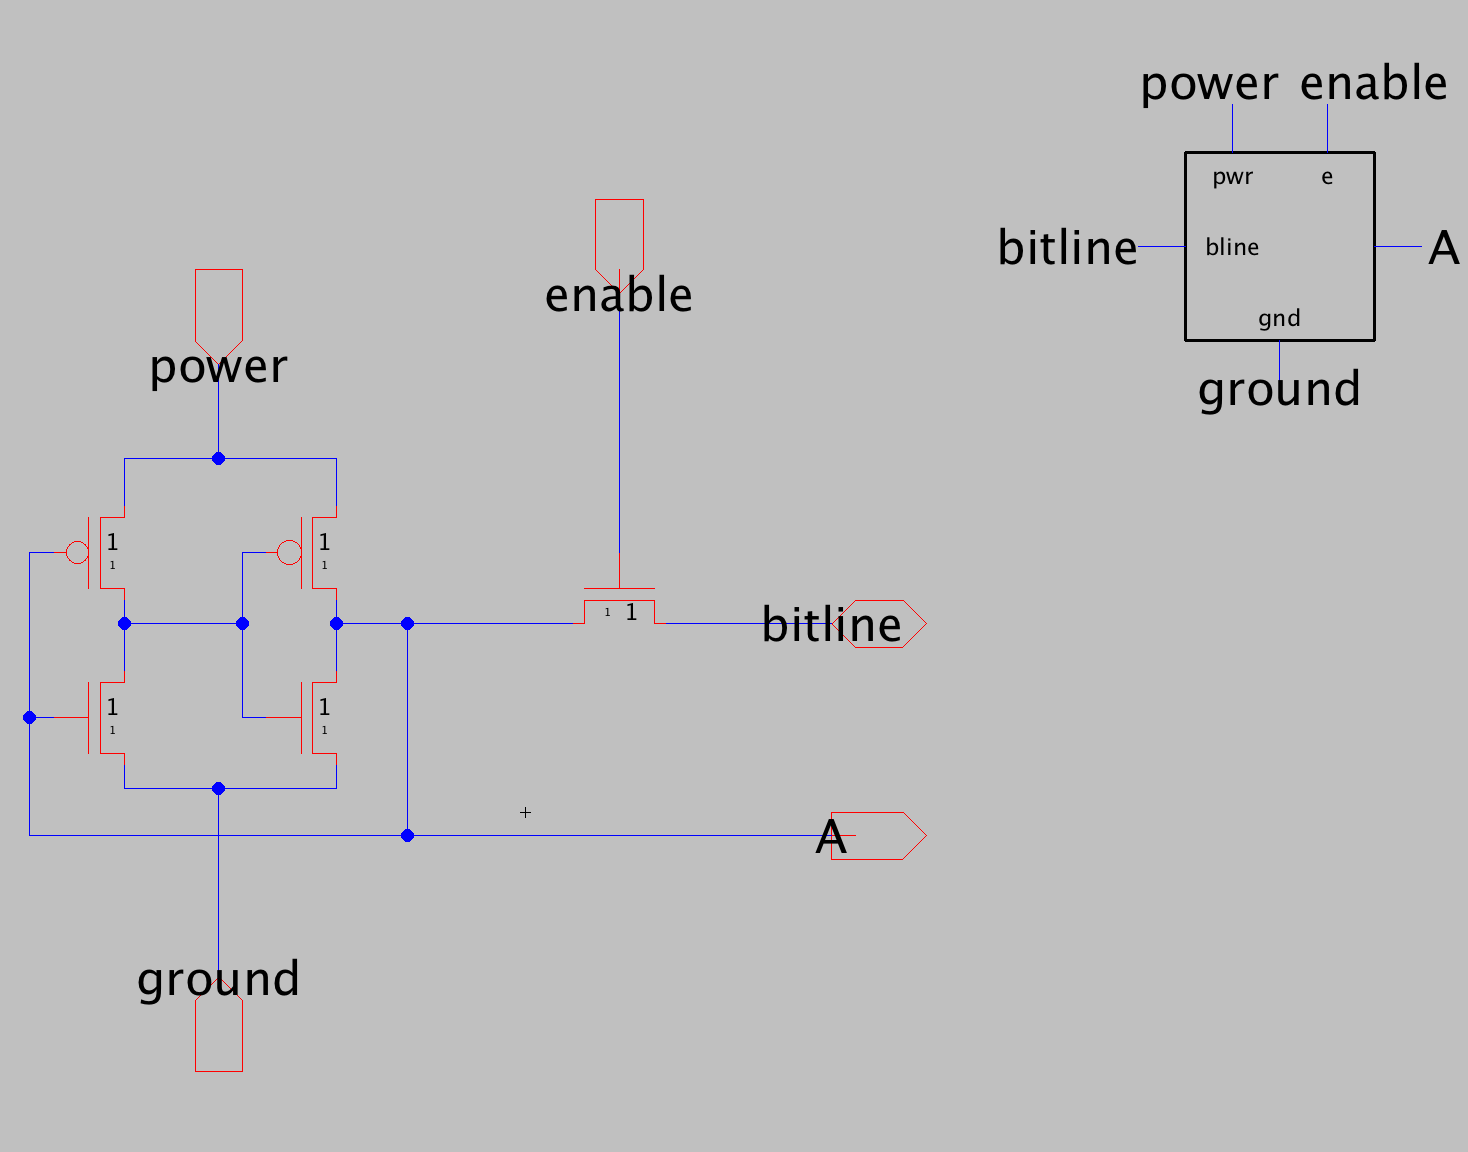
\includegraphics[scale=0.2]{5TCell}
	 \caption{5T Diagram}
	 \label{fig:5TCell}
 \end{figure}
 
To check the correctness of our design, we performed multiple tests. We created a special version of our ultimate memory cell with an output of A so that we can see the fluctuations of the held value. Below is the setup for our test bench.\\

\begin{figure}[H]
	\centering
	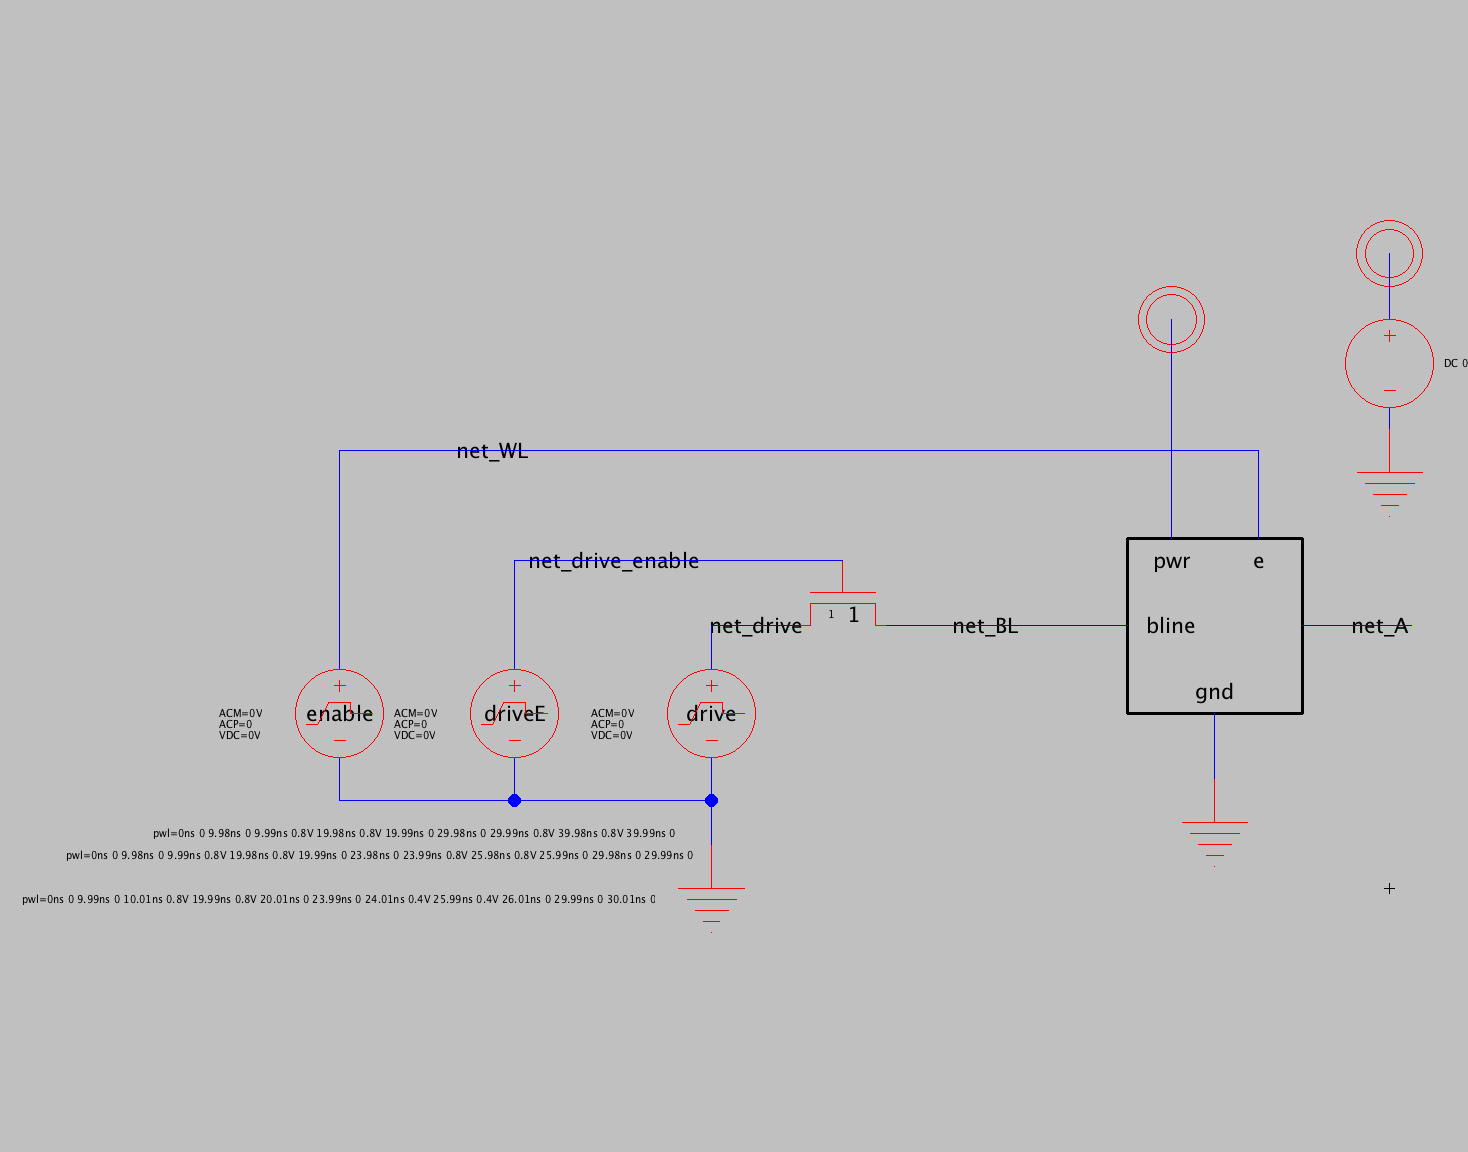
\includegraphics[scale=0.2]{5TCellTest}
	\caption{5TCell Test Bench}
	\label{fig:5TCellTest}
\end{figure}

 To start, we wrote a 1 to the memory cell and then read from the same cell. Below is the output waveform of that test.\\
 
 \begin{figure}[H]
	\centering
	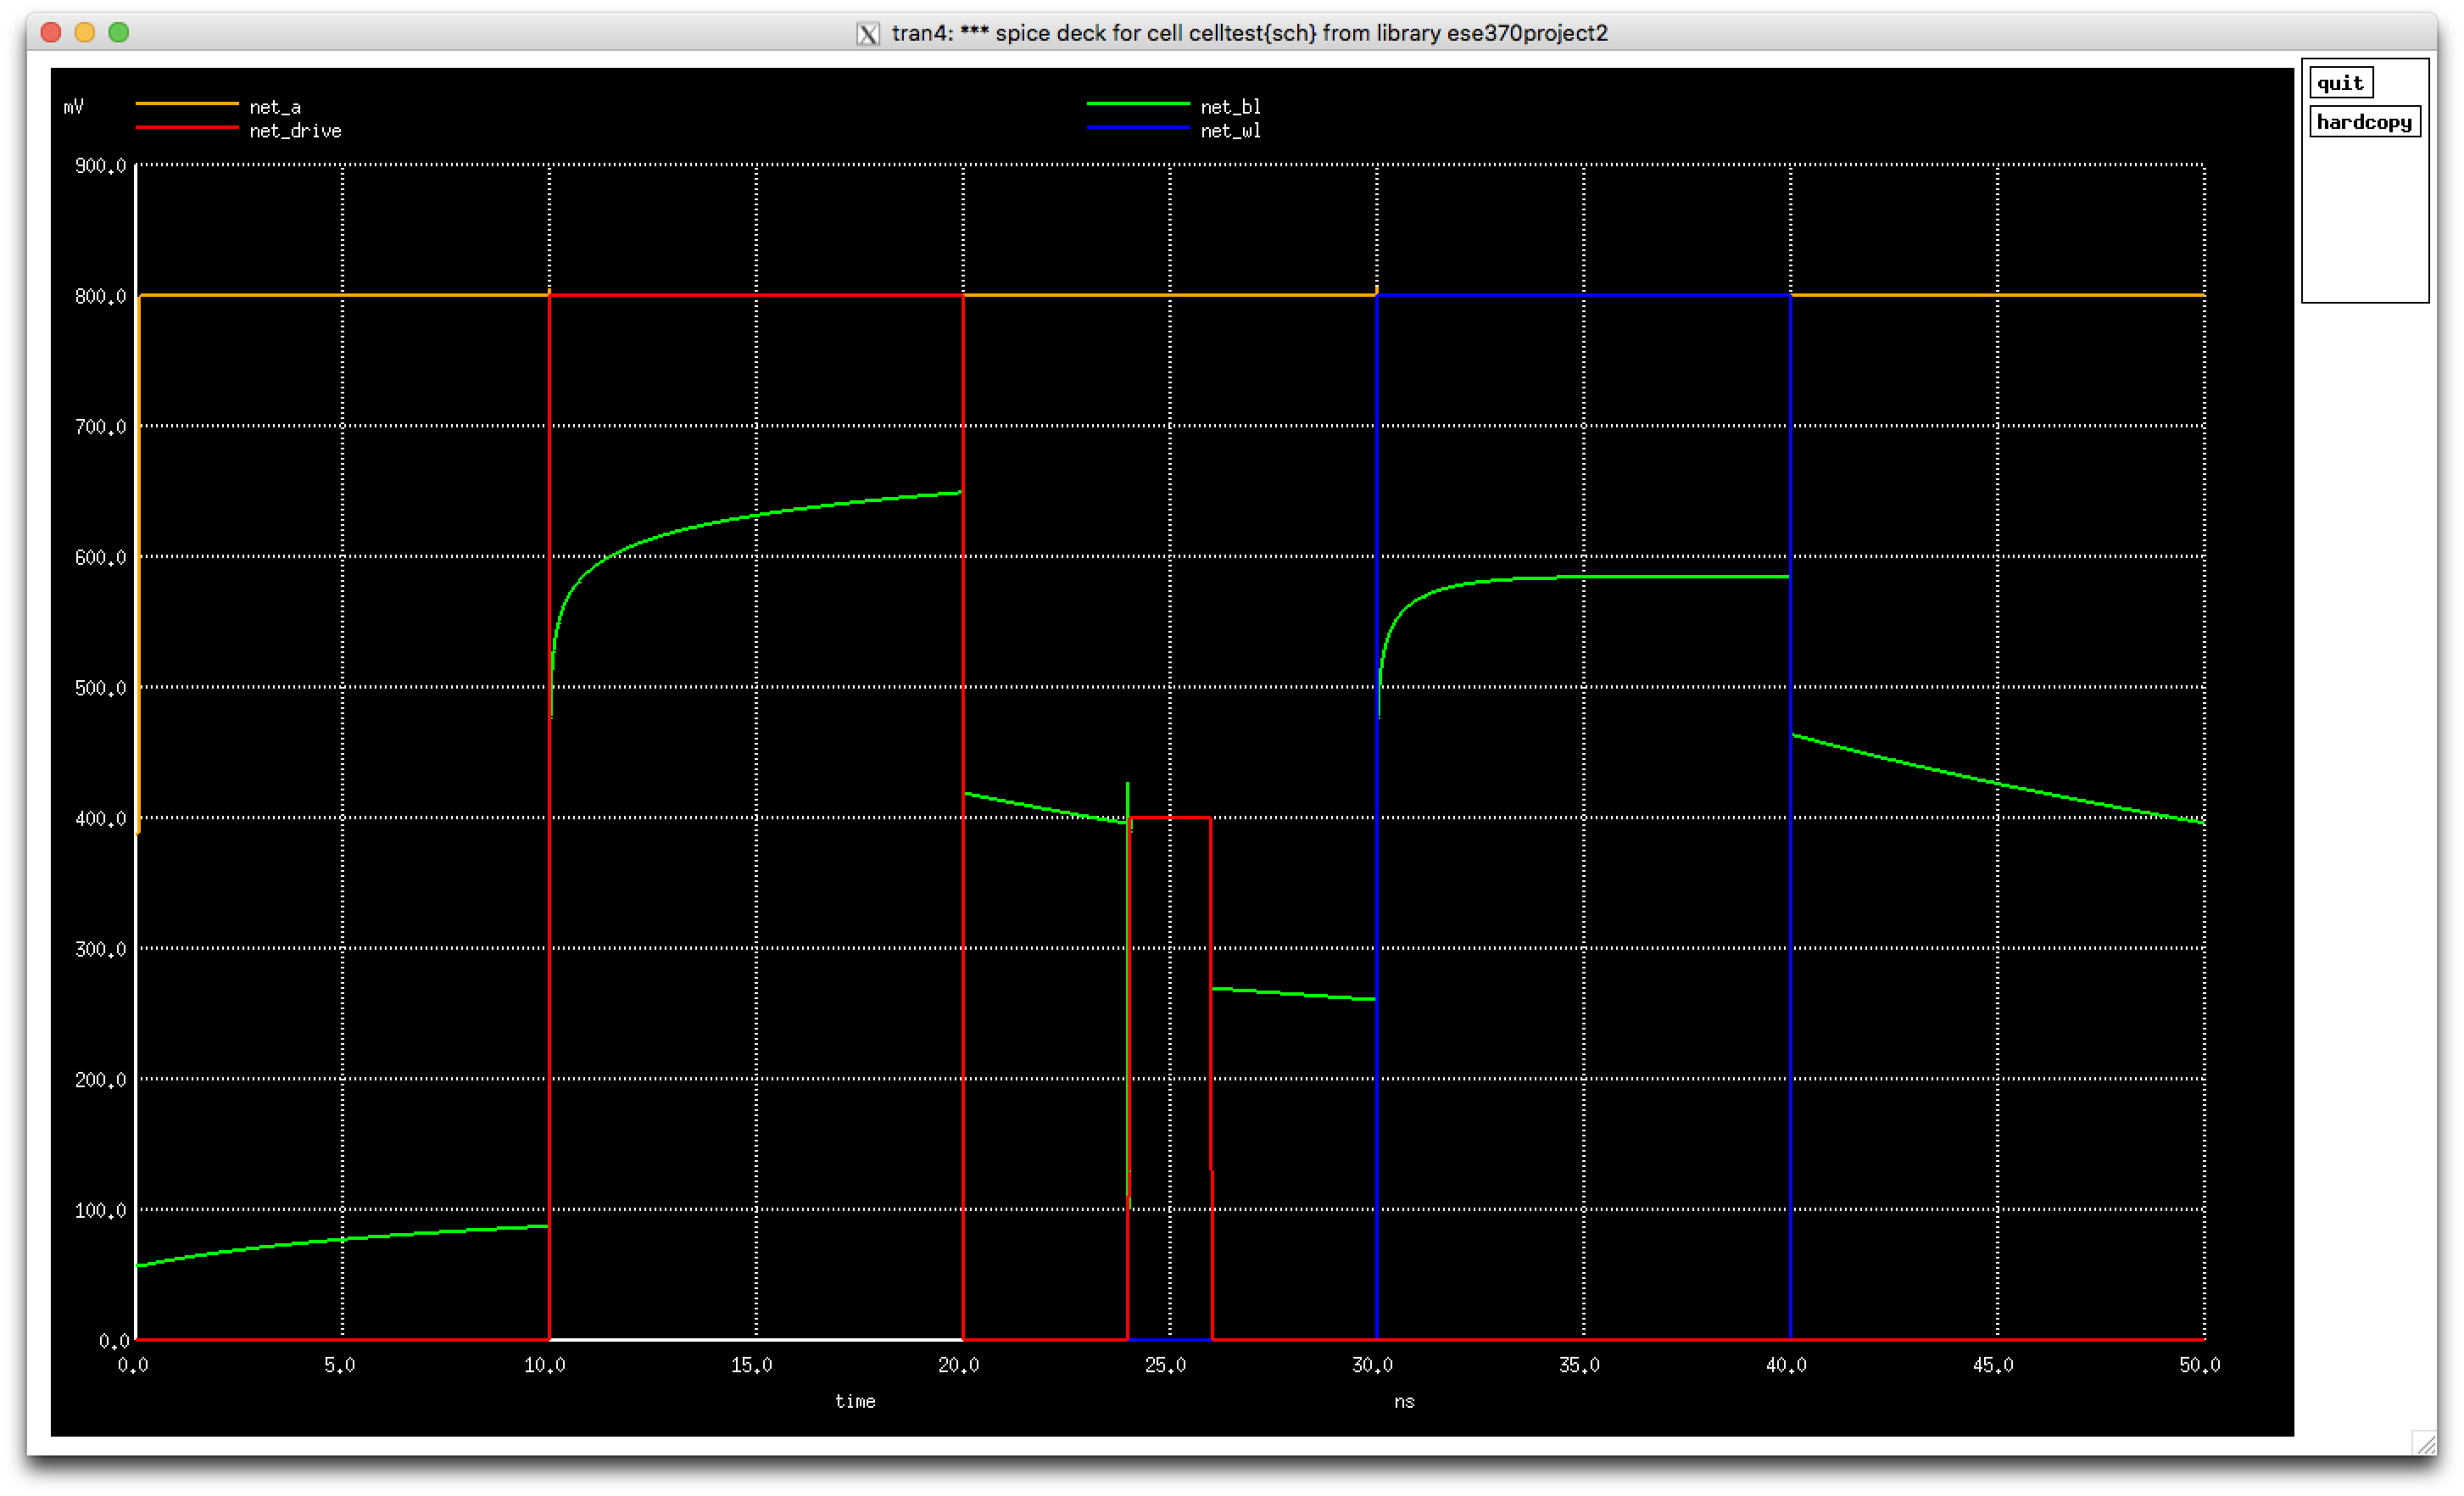
\includegraphics[scale=0.12]{5TWR1}
	\caption{5TCell Write/Read 1}
	\label{fig:5TWR1}
\end{figure}
We zoomed in on the point where \textbf{A} is written to a 1 which is shown below.\\

 \begin{figure}[H]
	\centering
	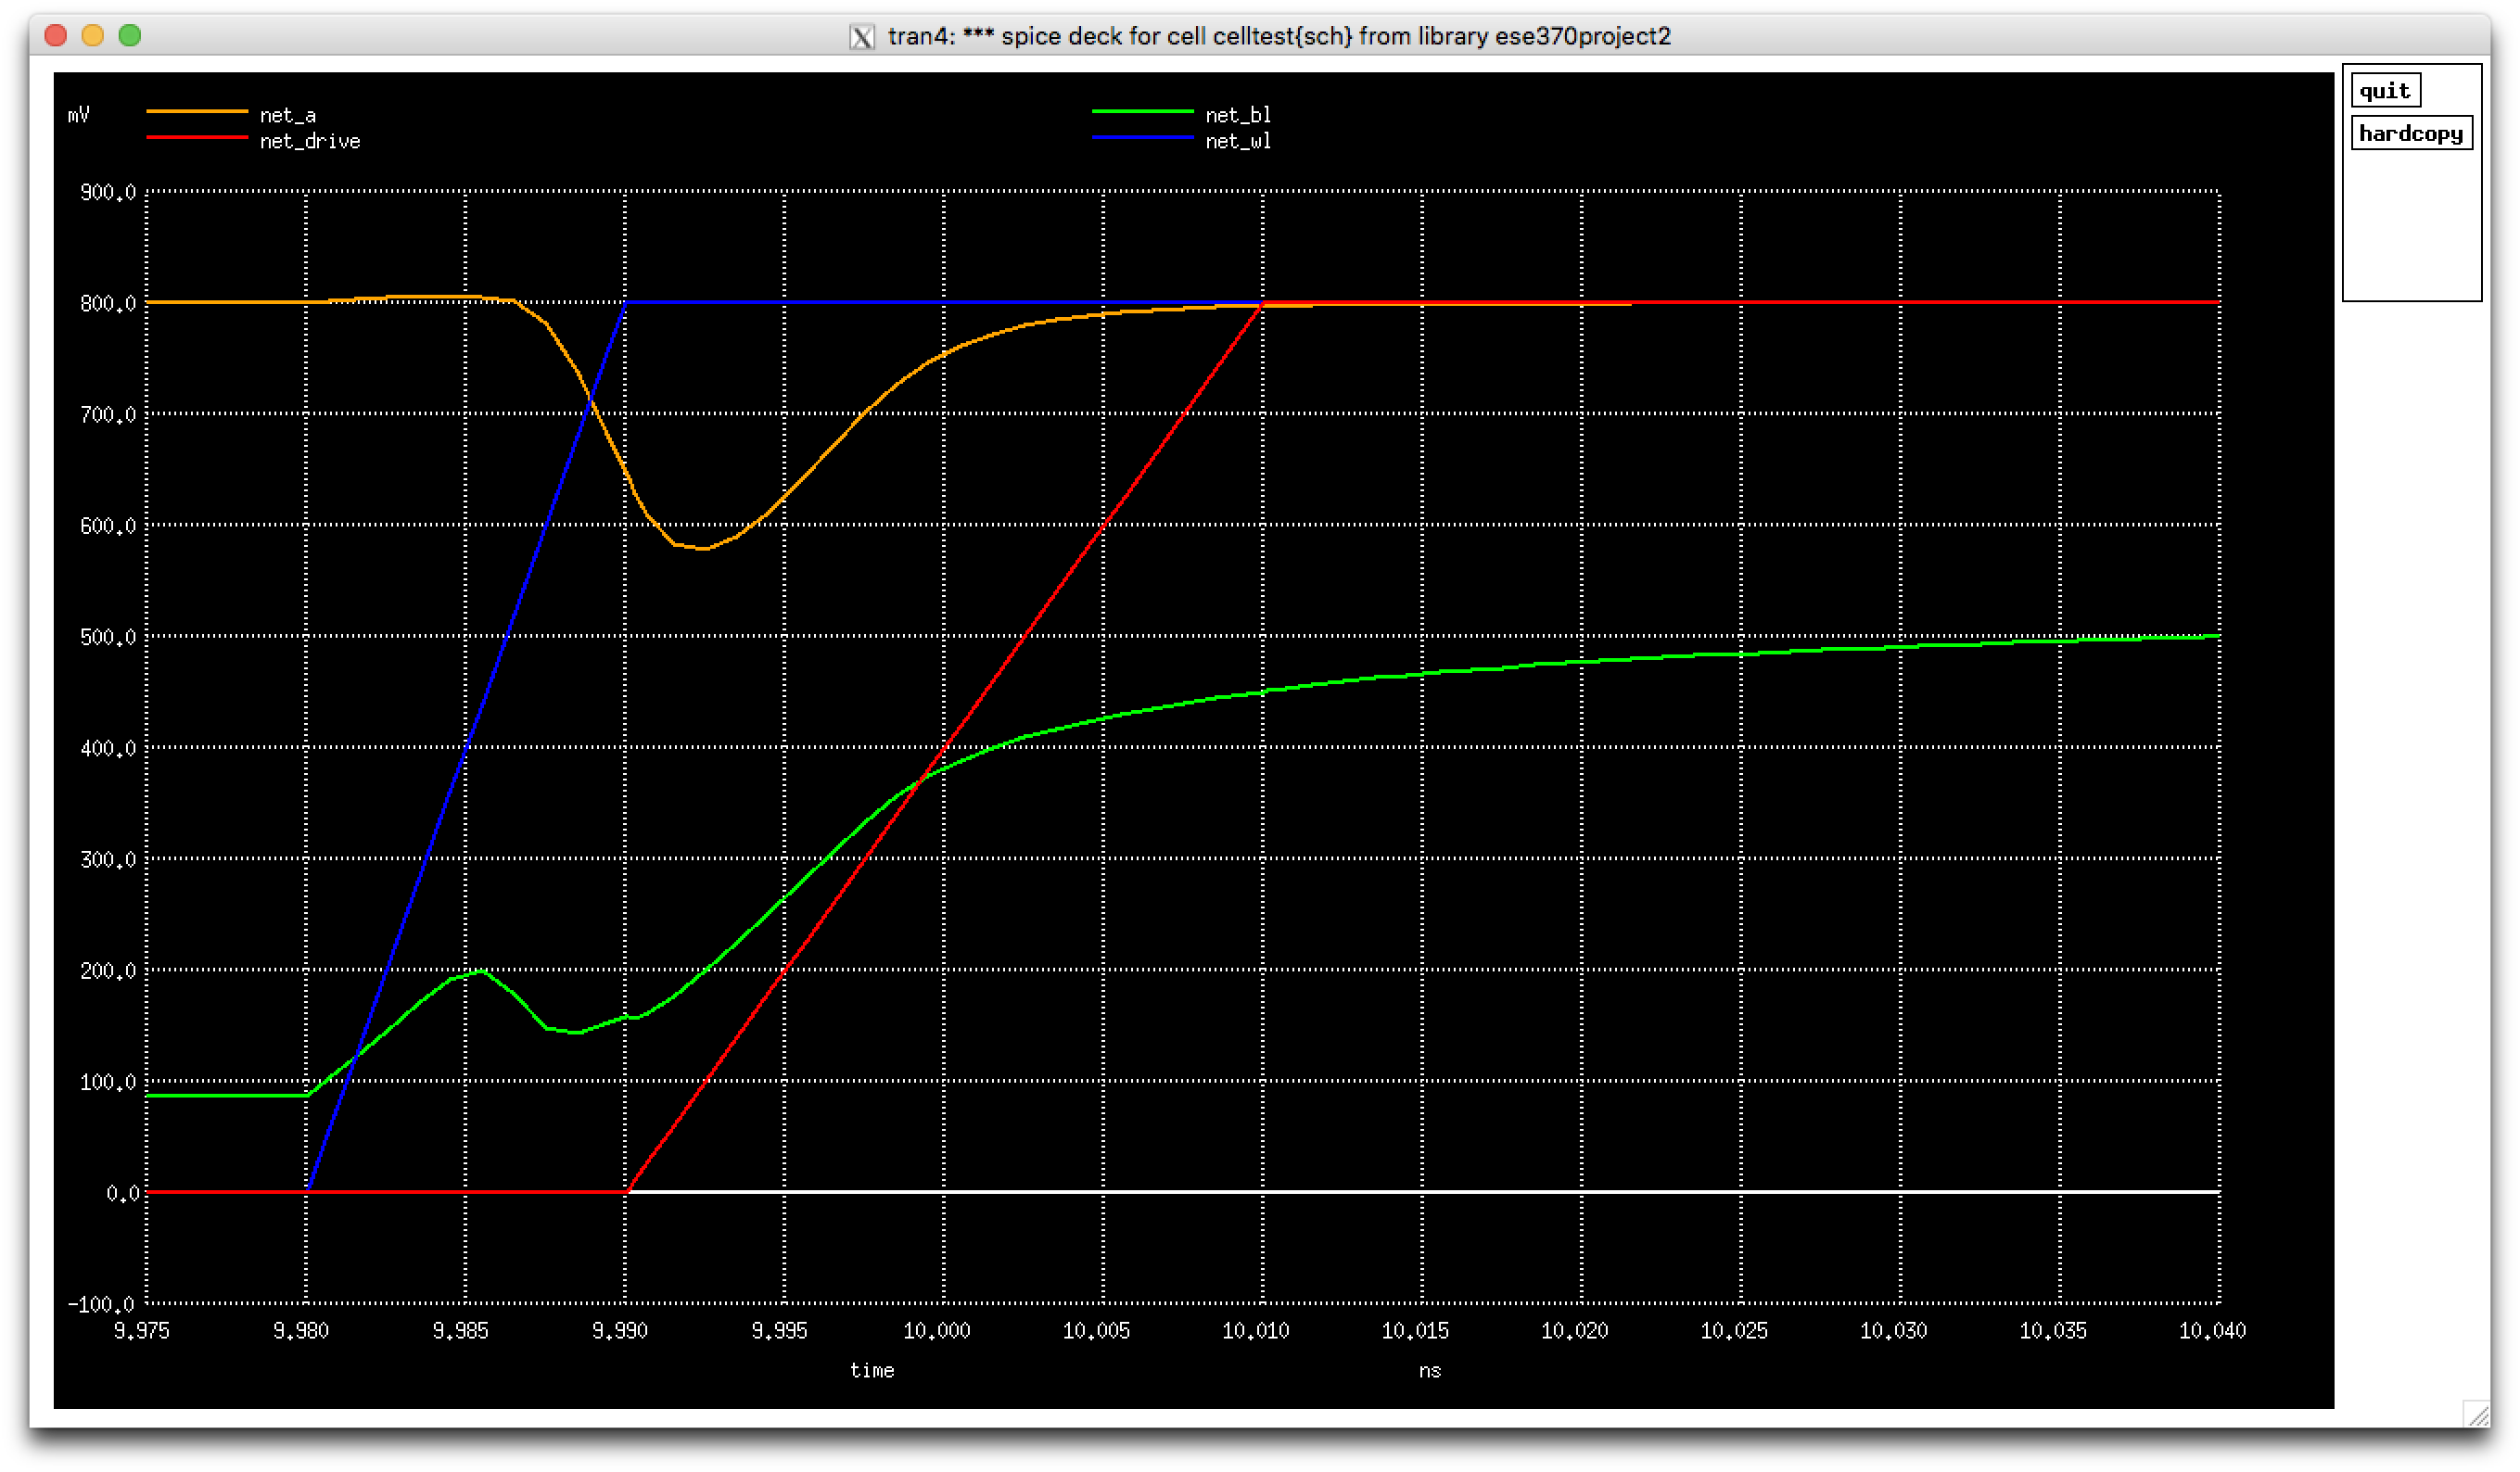
\includegraphics[scale=0.12]{5TWrite1}
	\caption{5TCell Write 1}
	\label{fig:5TWrite1}
\end{figure}

Here you can see the slight dip in \textbf{A} before the drive line goes high. Eventually as the driving signal goes high, \textbf{A} responds accordingly. We also checked the zoomed in part of the read operation and have put that in below.

 \begin{figure}[H]
	\centering
	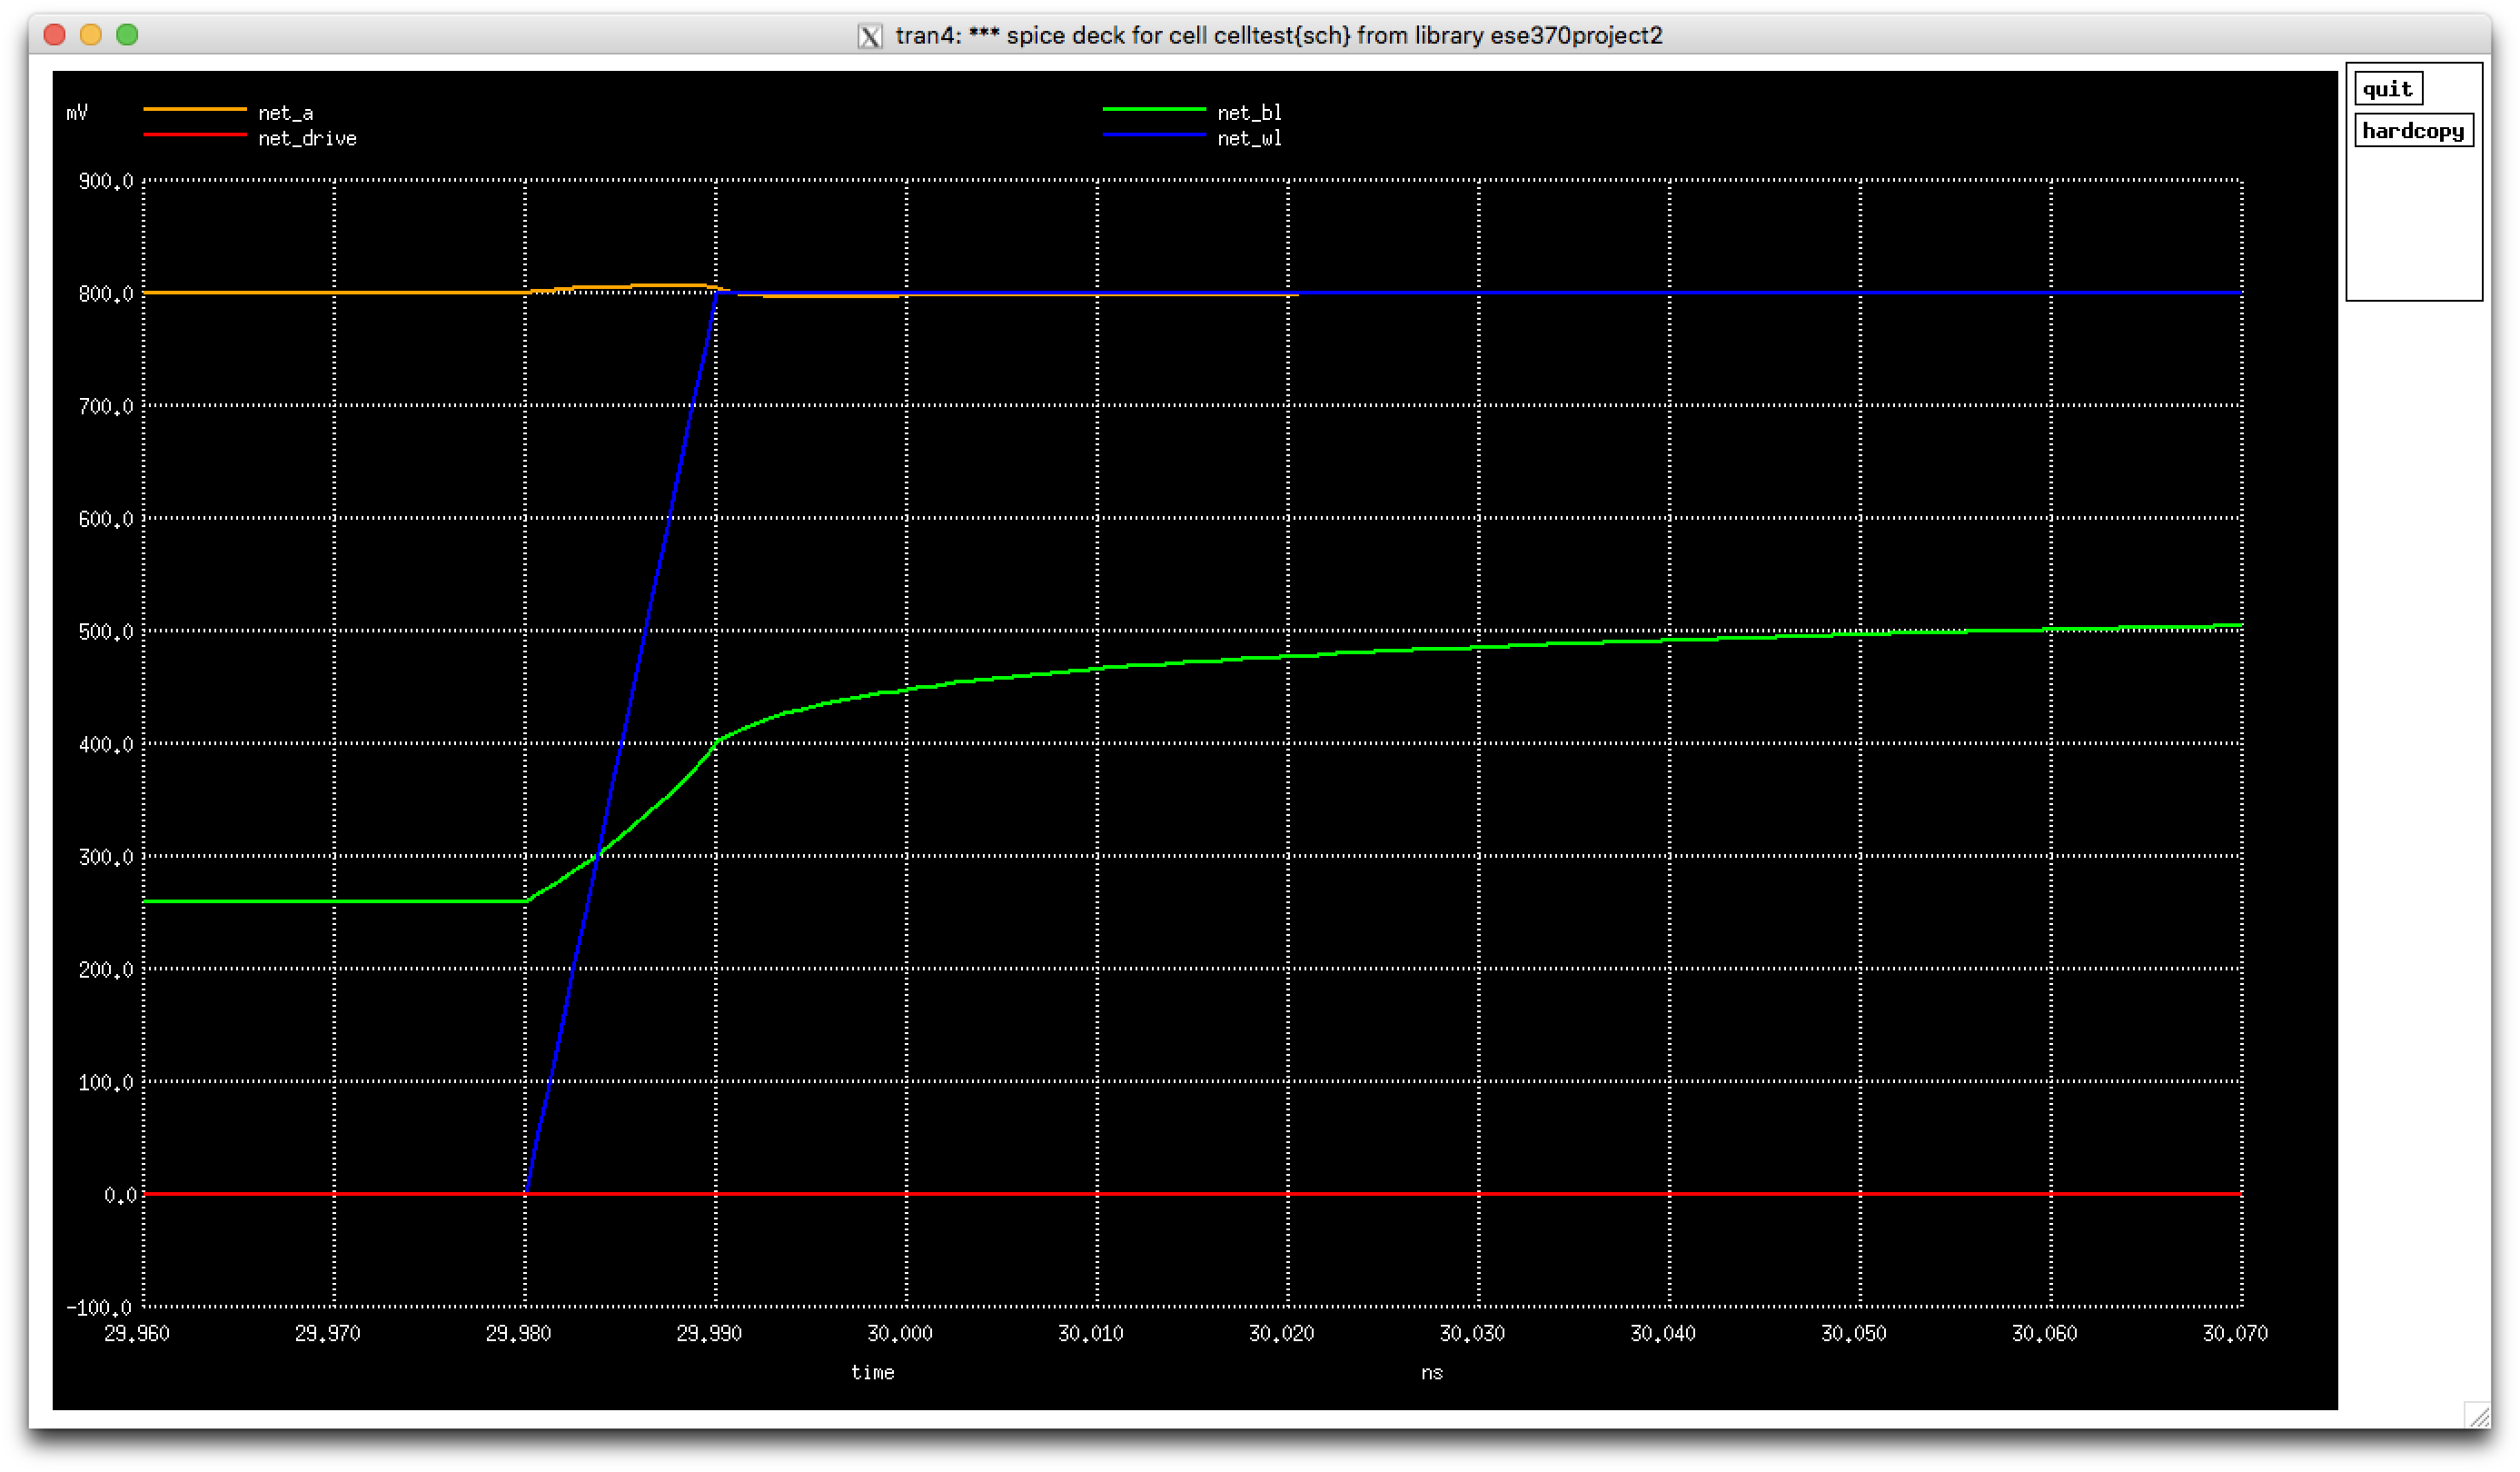
\includegraphics[scale=0.12]{5TRead1}
	\caption{5TCell Read 1}
	\label{fig:5TRead1}
\end{figure}

To check the correctness of our memory cell, we also had to check that if we performed a back-to-back read operation after a write, that A didn't flip as a result. Below is our test to check in case \textbf{A} = 1.

 \begin{figure}[H]
	\centering
	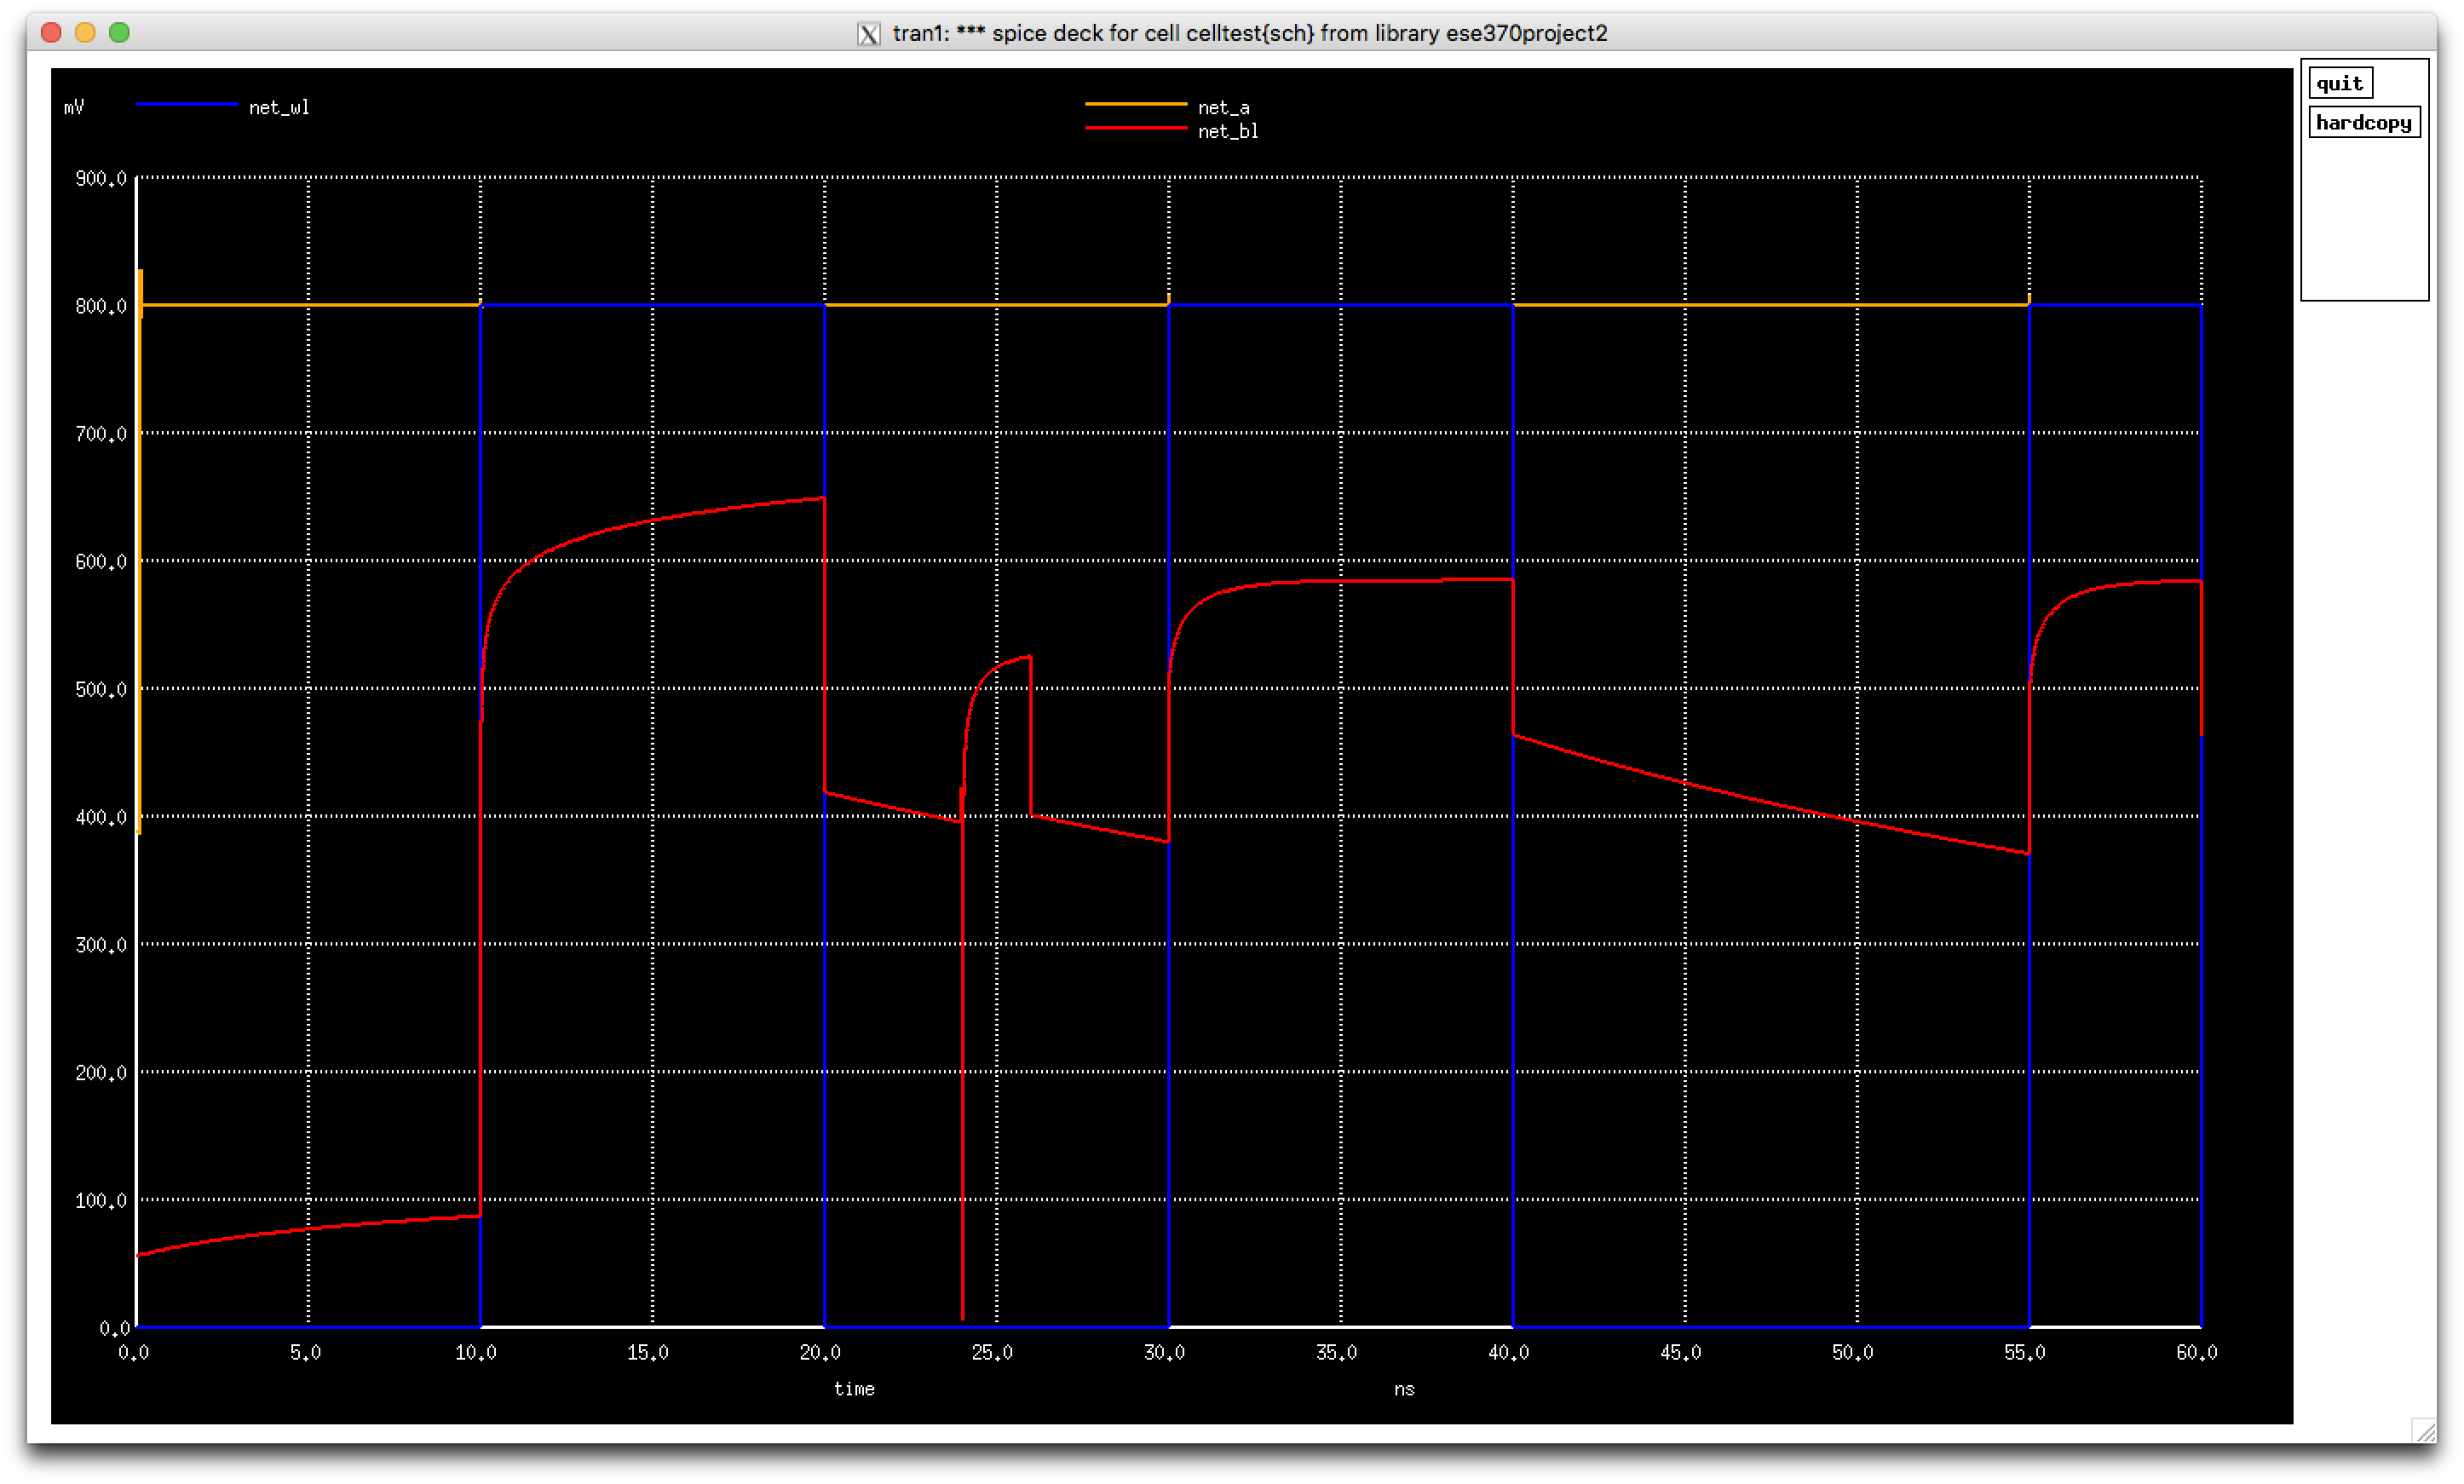
\includegraphics[scale=0.12]{5TDoubleRead1}
	\caption{5TCell Back-to-Back Read 1}
	\label{fig:5TBackToBack1}
\end{figure}

We also checked the back-to-back read operation when \textbf{A} = 0.

 \begin{figure}[H]
	\centering
	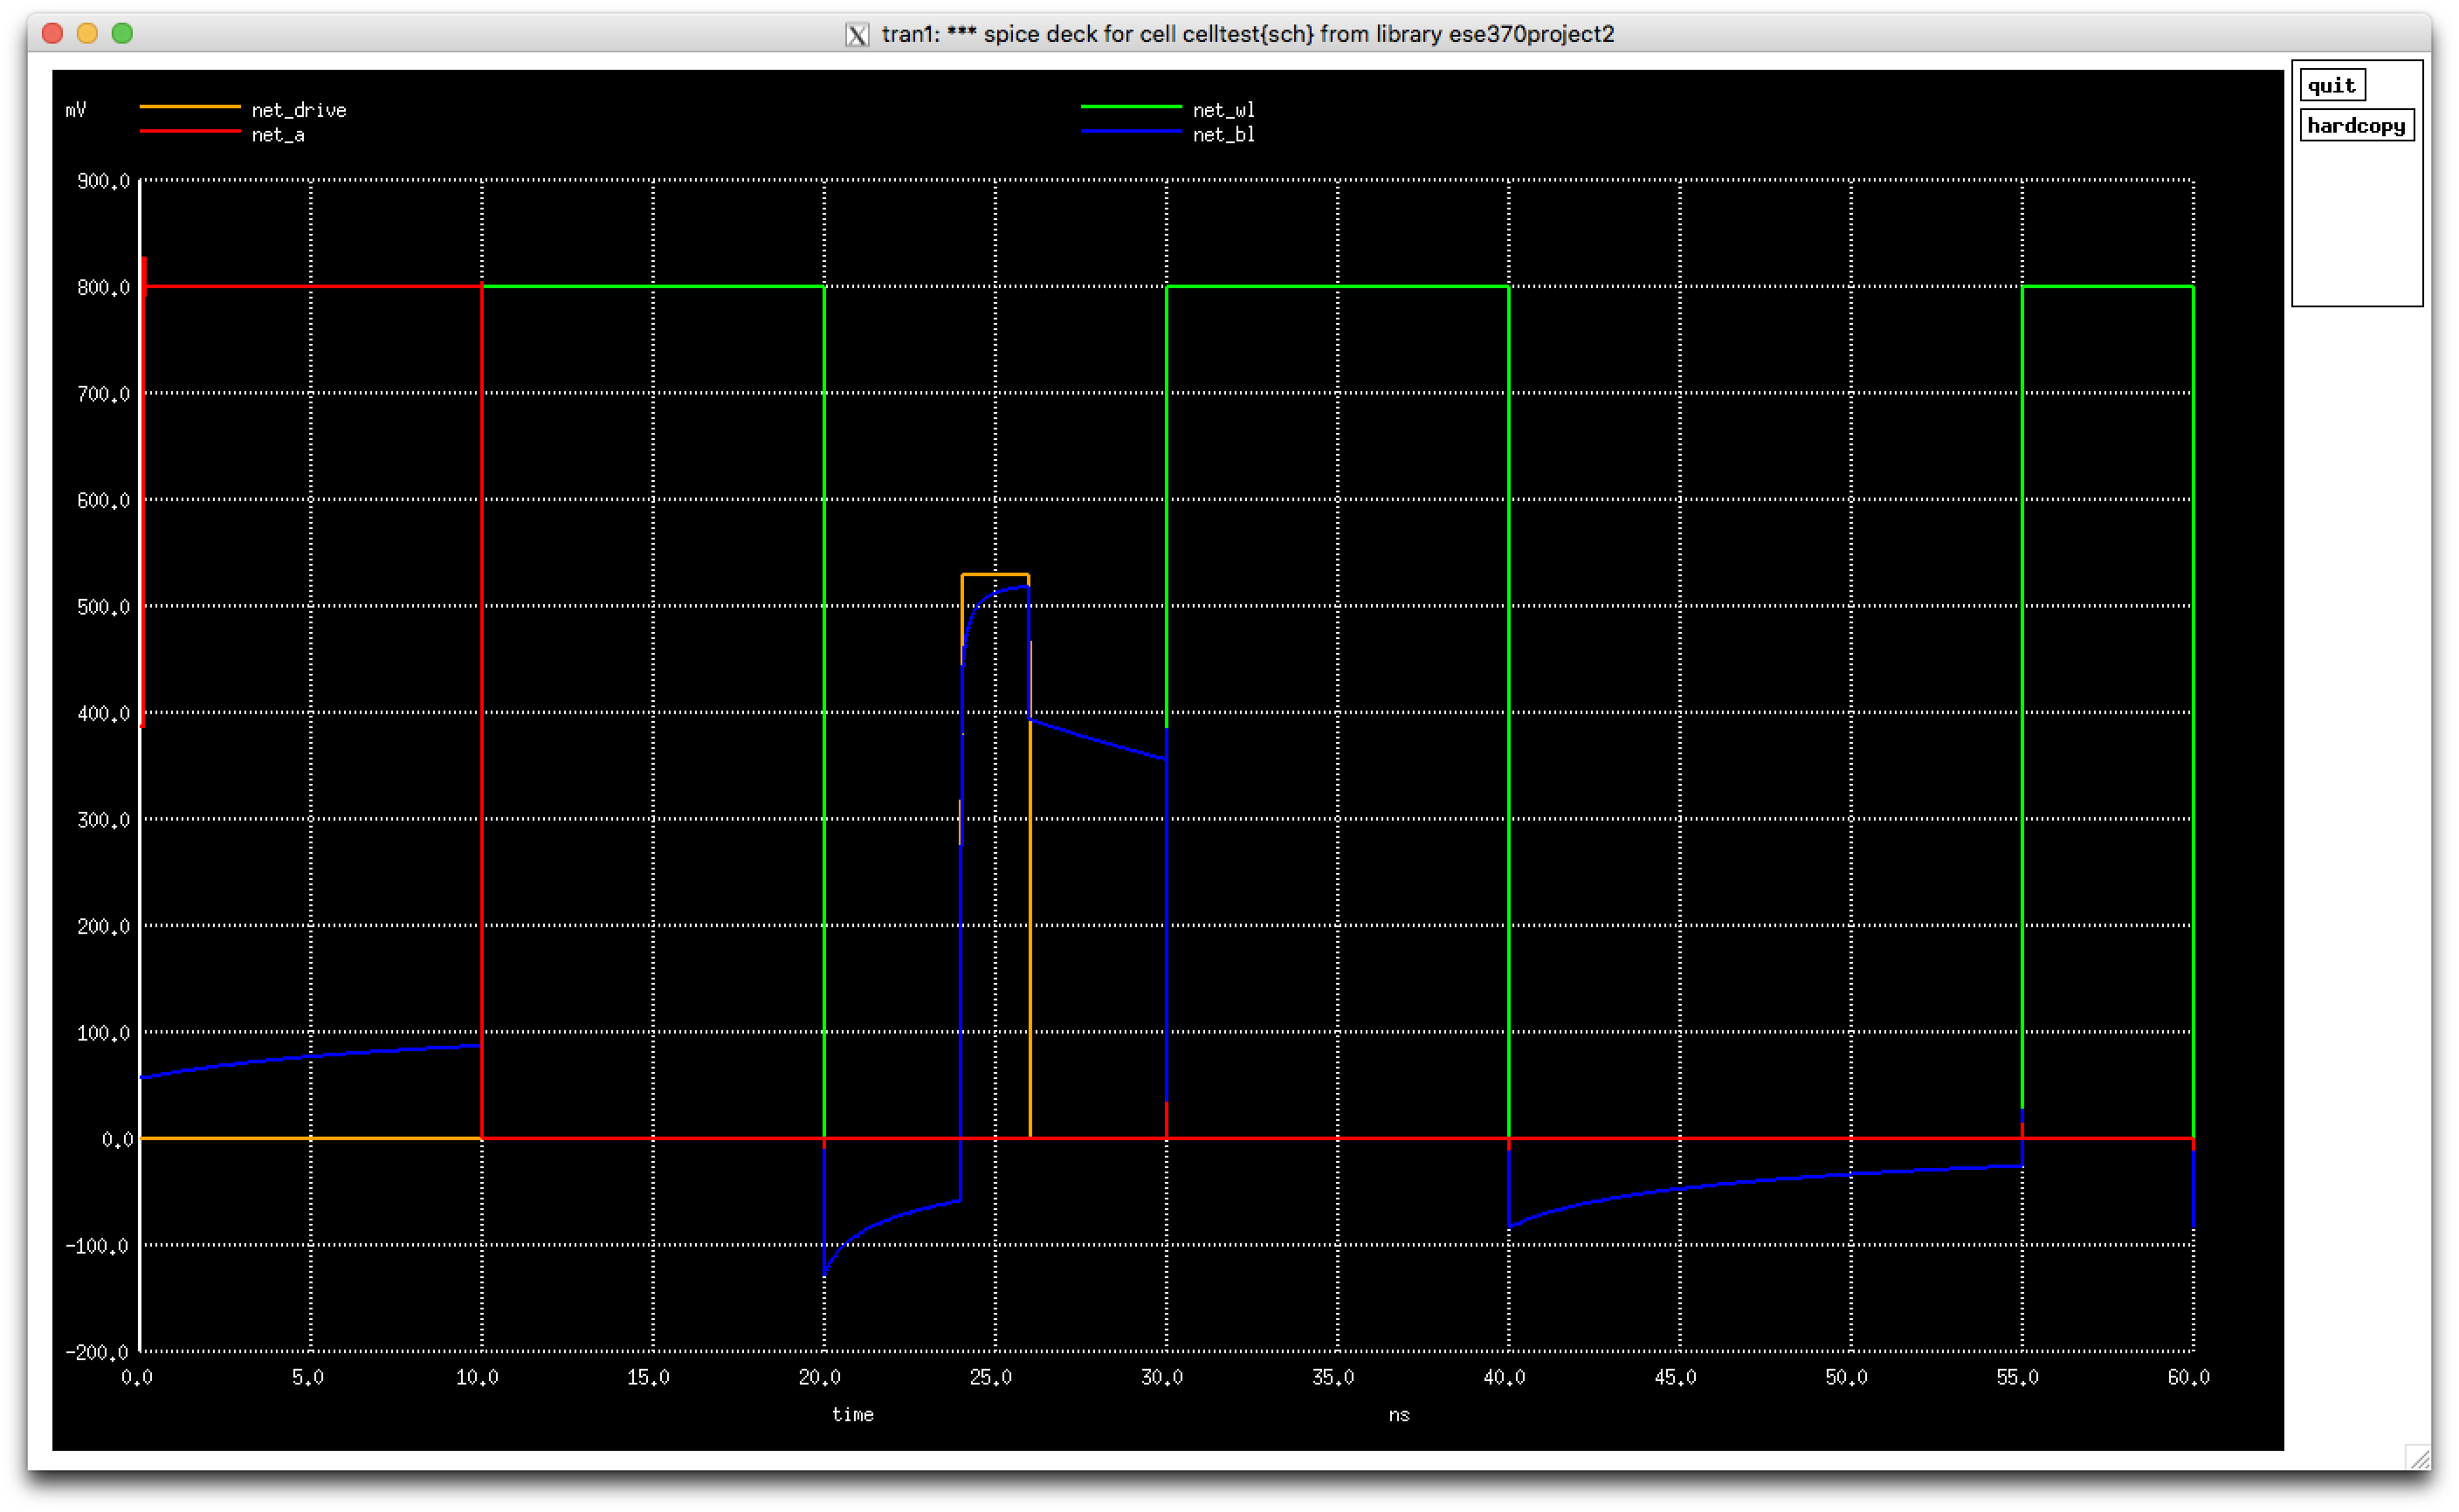
\includegraphics[scale=0.12]{5TDoubleRead0}
	\caption{5TCell Back-to-Back Read 0}
	\label{fig:5TBackToBack0}
\end{figure}

As the figure shows, \textbf{A} stays stable at 0.

\subsubsection{Sense Amplifier}
Sense amp stuff pls
\subsubsection{$\frac{\textbf{Vdd}}{\textbf{2}}$ Reference Generator}
Below is the circuit for our voltage reference ($\frac{\textbf{Vdd}}{\textbf{2}}$) generator as given in the assignment prompt.

\begin{figure}[H]
	\centering
	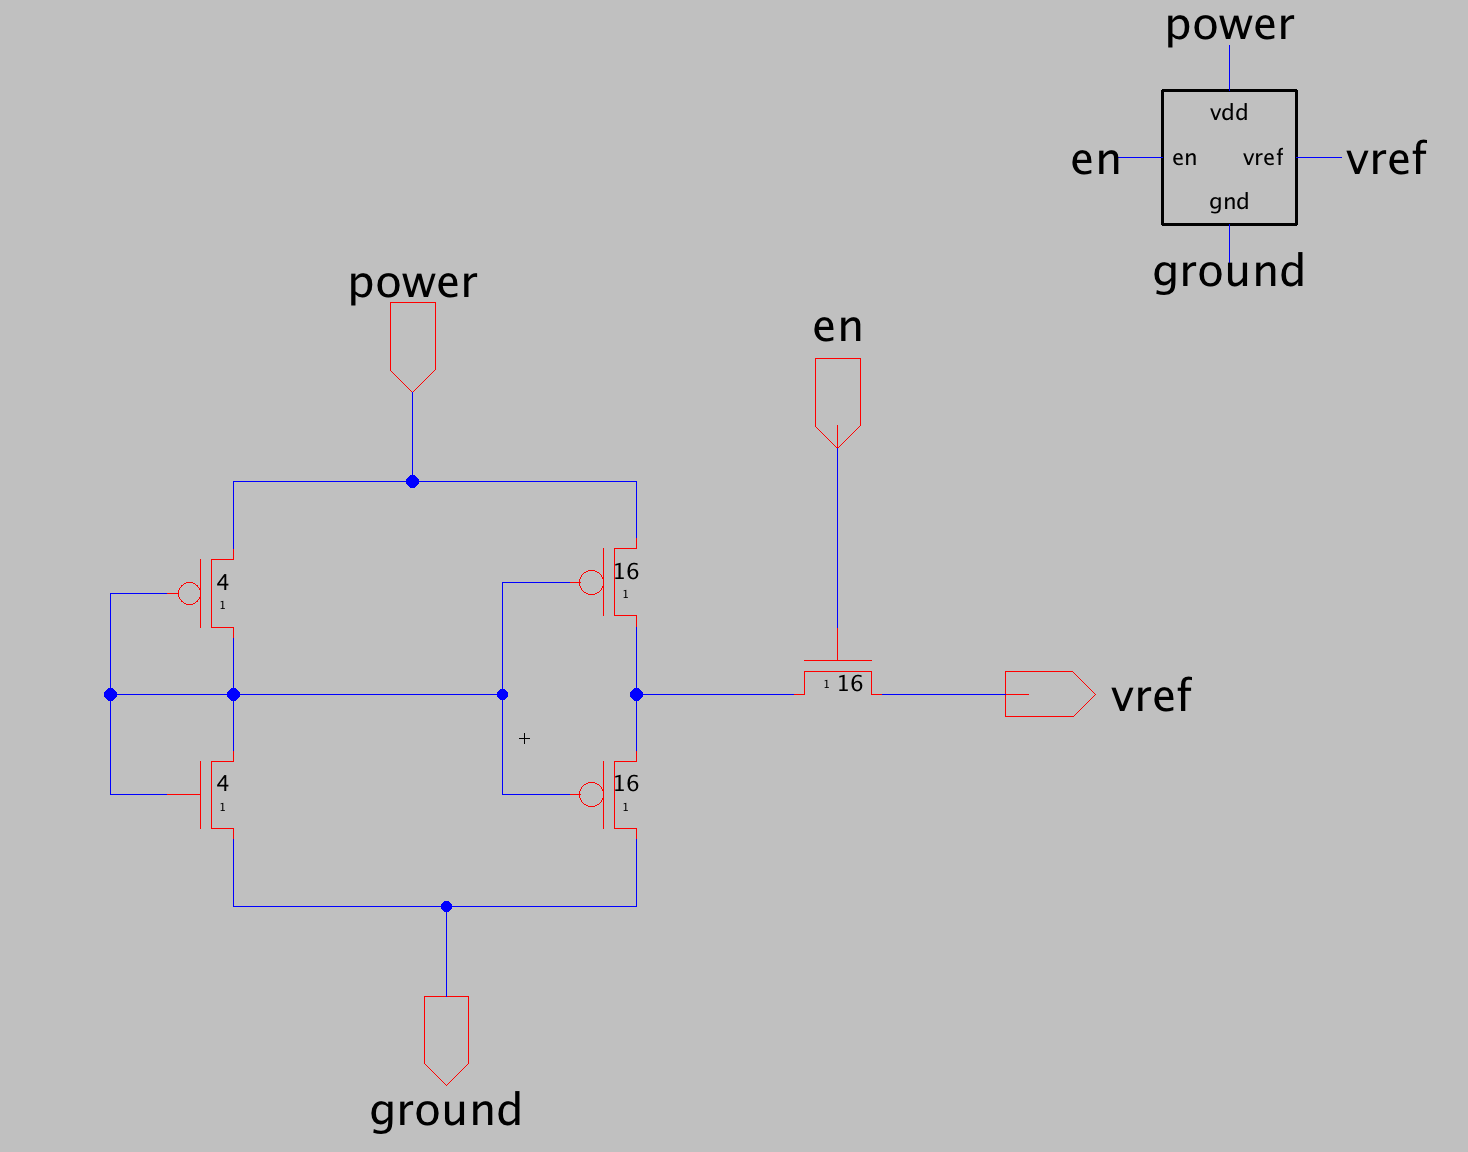
\includegraphics[scale=0.17]{vRefGen}
	\caption{Voltage Reference Generator}
	\label{fig:vRefGen}
\end{figure}

We tested the circuit with the below test bench.\\

\begin{figure}[H]
	\centering
	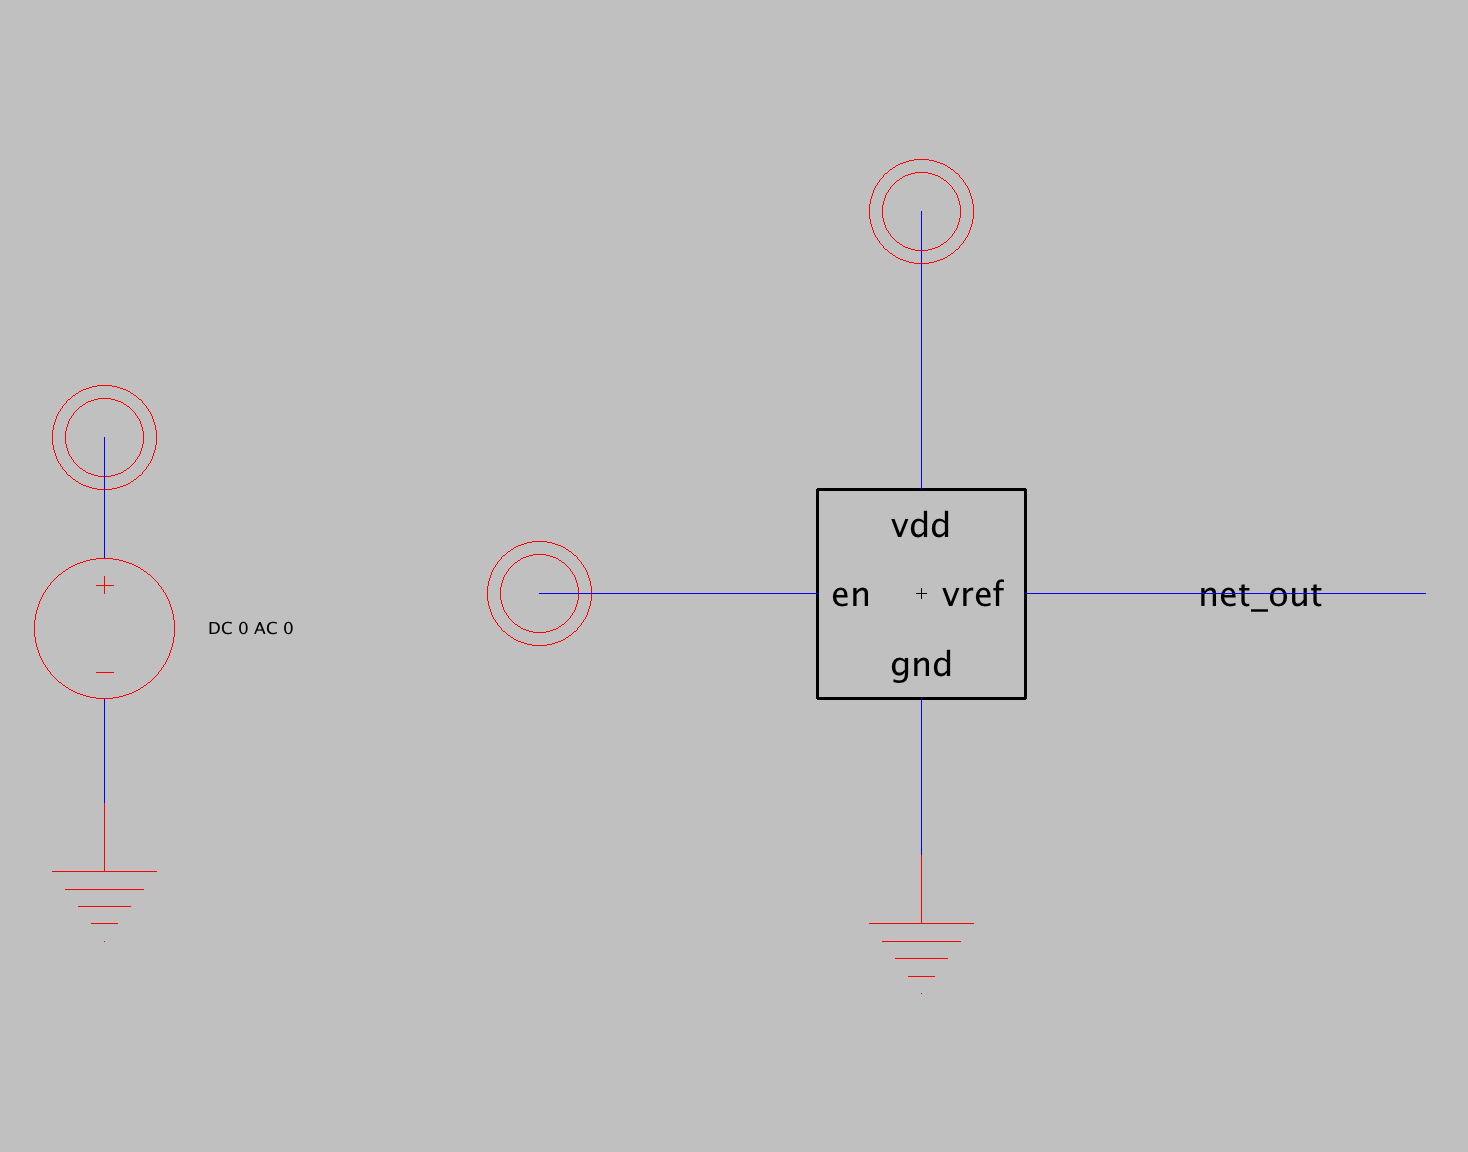
\includegraphics[scale=0.17]{vRefTest}
	\caption{Voltage Reference Generator Test Bench}
	\label{fig:vRefTest}
\end{figure}

With that test bench we generated the below waveform.\\

\begin{figure}[H]
	\centering
	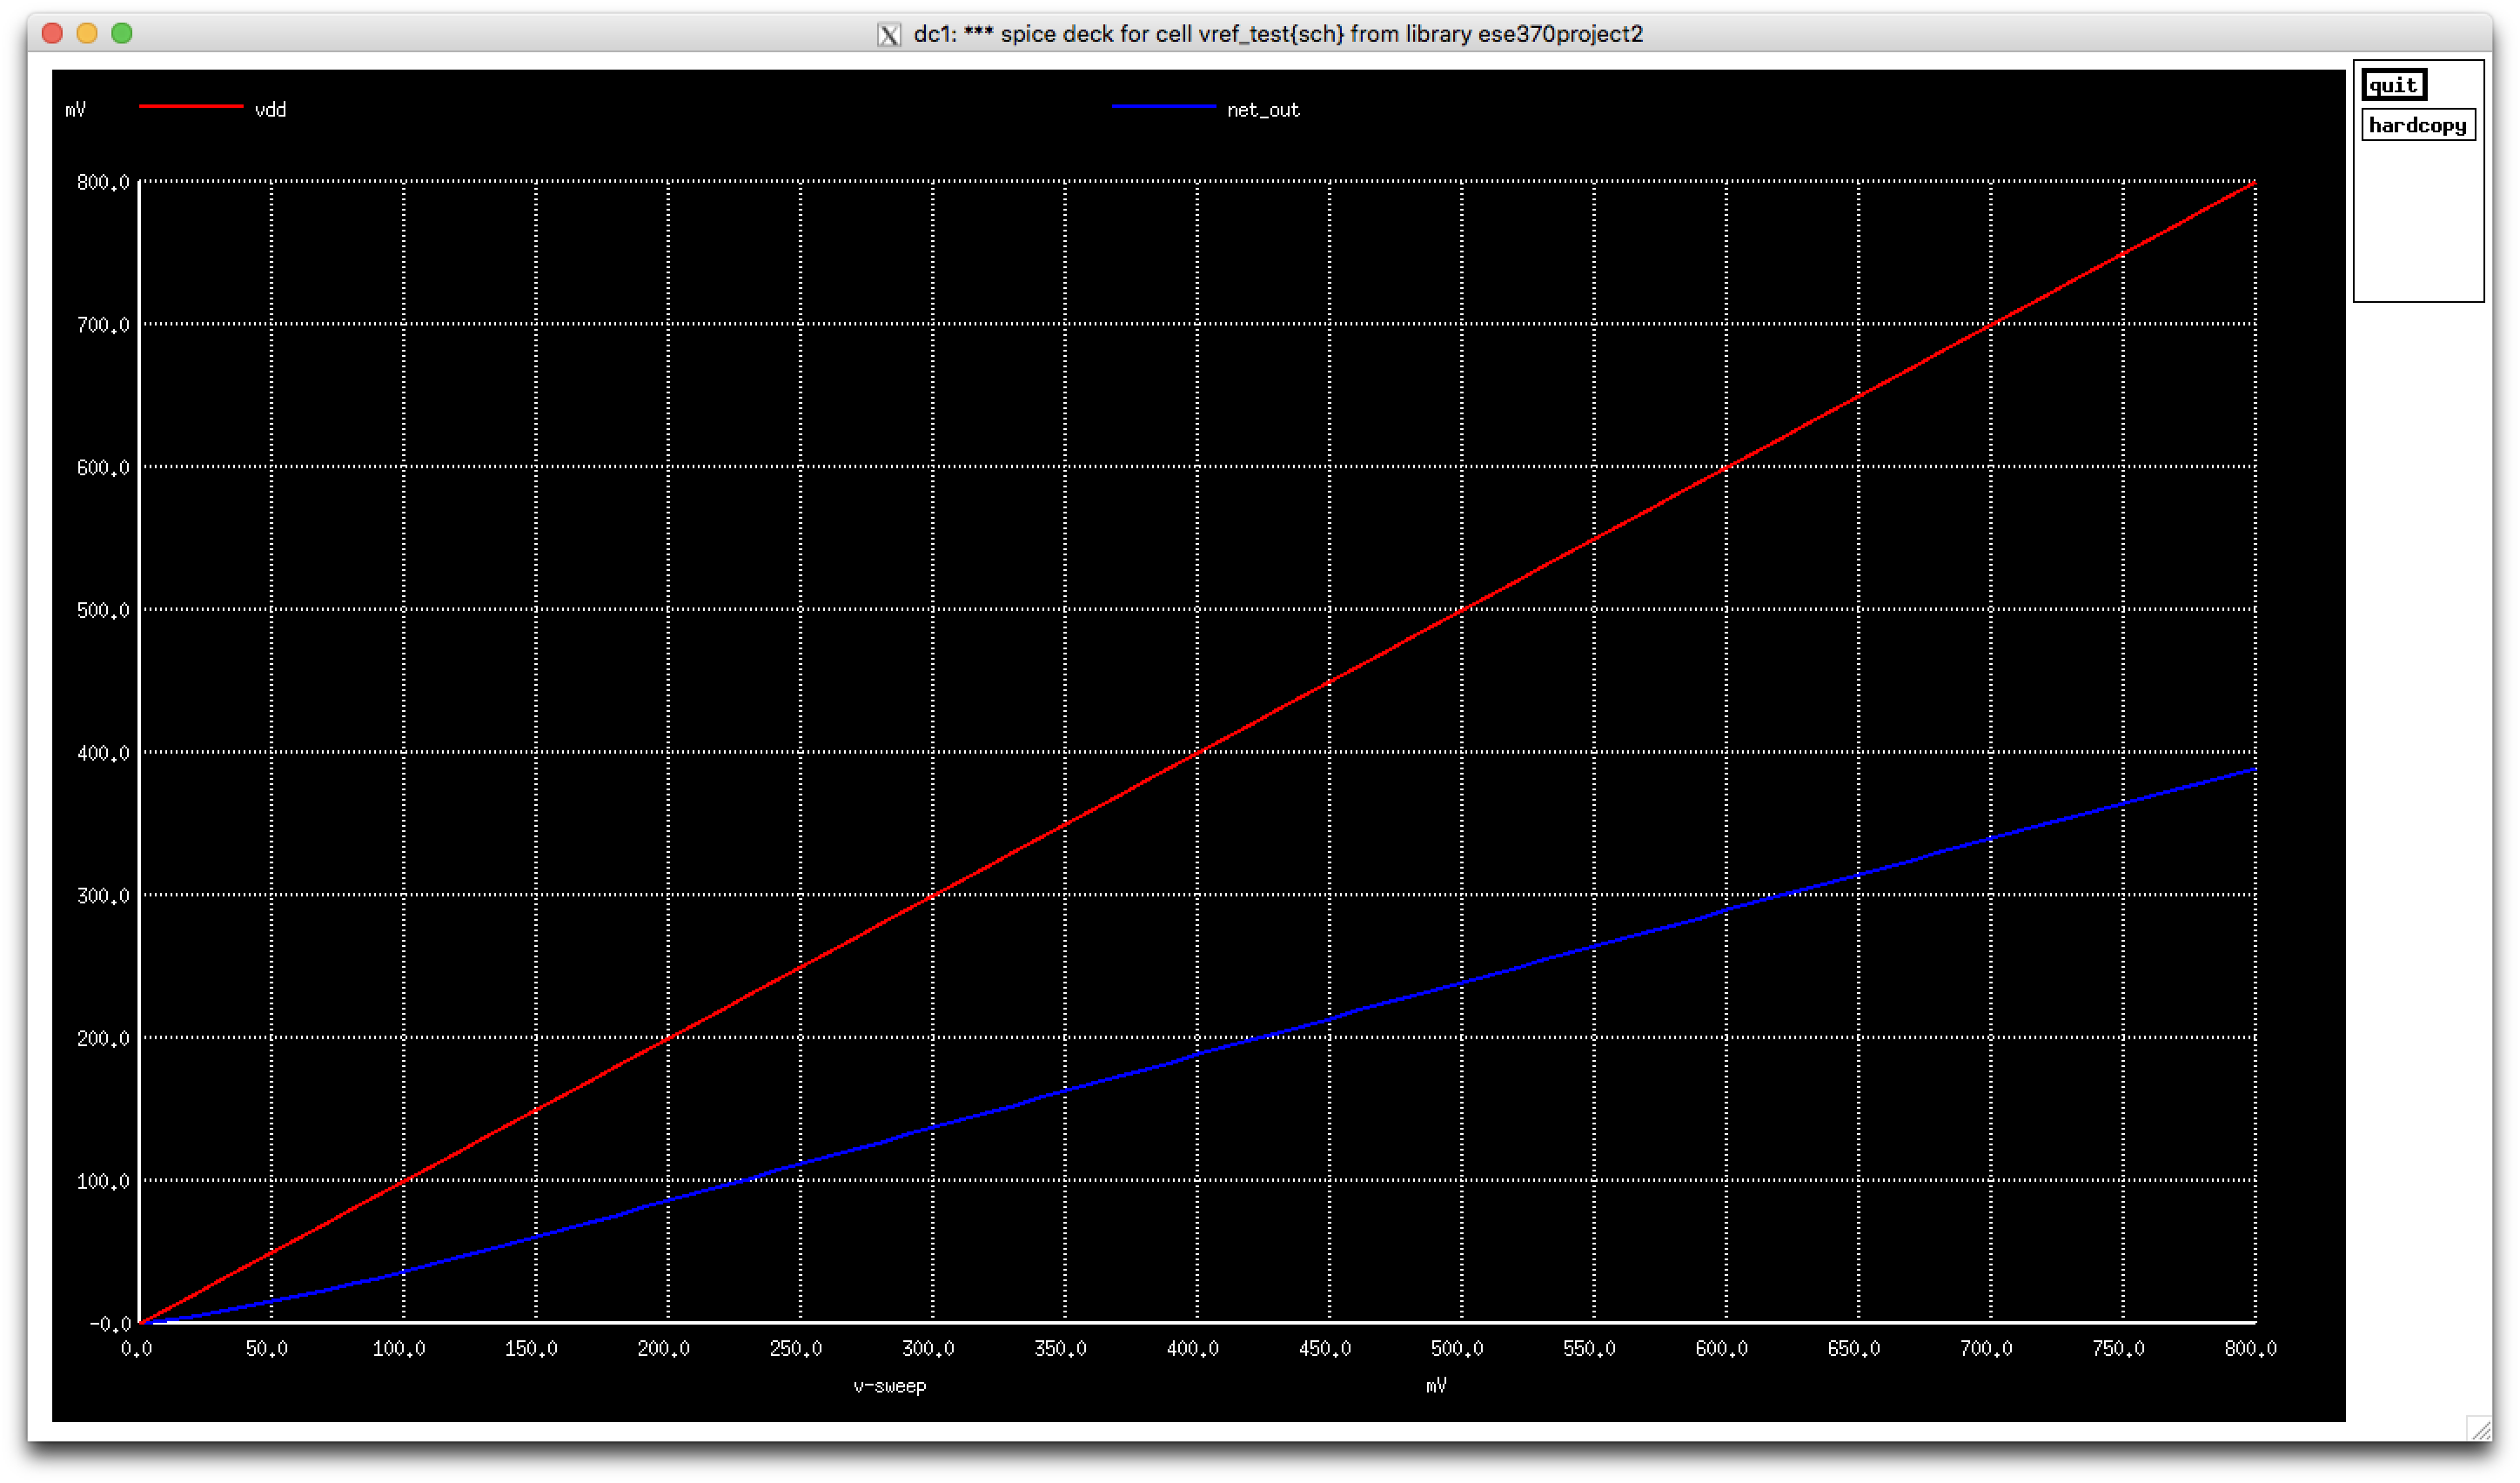
\includegraphics[scale=0.1]{vRefTestWave}
	\caption{Voltage Reference Generator Test Bench Waveform}
	\label{fig:vRefTestWave}
\end{figure}

You can see that for every given value of $V_{dd}$, the output is (or is very very close to) half of $V_{dd}$.

\subsubsection{Bit Line Driver}
Schematic
\subsubsection{Complete Bit Line}
\textbf{Correctness}

\subsection{Calculations}
\subsubsection{Capacitance}
Bitline with drive and pre-charge enable transistors disabled:
\begin{align*}
C_{total} &= C_{pre-charger} + C_{driver} + 16 C_{memcell} + C_{senseamp}\\
&= 16 \gamma C_0 + W_{} + 16 C_{memcell} + C_{senseamp}
\end{align*}

\subsubsection{Timing}

\subsubsection{Energy}
Energy calculations



\section{Metrics}
\label{sec:mtrics}

\subsection{Area}
\begin{enumerate}
\item memory cell area
\item total area
\end{enumerate}

\subsection{Energy}
\subsubsection{Enqueue Energy}
To test enqueue energy, we looked at both the energy to transition from $0x0000$ to $0xFFFF$ and vice-versa. The reported values are below with the test schematic shown in Figure \ref{fig: todo} and the resulting waveforms in Figure \ref{fig: todo} and Figure \ref{fig: todo} respectively.
$$0x0000 \rightarrow 0xFFFF = xW$$
$$0xFFFF \rightarrow 0x0000 = yW$$
\subsubsection{Dequeue Energy}
This was a test for dequeueing a single value. We tested both $0x0000$ and $0xFFFF$
$$0x0000 = xW\textnormal{ (shown in Figure \ref{fig: todo})}$$
$$0xFFFF = yW\textnormal{ (shown in Figure \ref{fig: todo})}$$

\subsubsection{Enqueue/Dequeue Energy}
The energy for a single enqueue and dequeue is as follows:

\newpage
\section{Some LaTeX tips}
\label{sec:latex}
\subsection{How to Include Figures}

First you have to upload the image file (JPEG, PNG or PDF) from your computer to writeLaTeX using the upload link the project menu. Then use the includegraphics command to include it in your document. Use the figure environment and the caption command to add a number and a caption to your figure. See the code for Figure \ref{fig:frog} in this section for an example.

% \begin{figure}
% \centering
% \includegraphics[width=0.3\textwidth]{frog.jpg}
% \caption{\label{fig:frog}This frog was uploaded to writeLaTeX via the project menu.}
% \end{figure}

\subsection{How to Make Tables}

Use the table and tabular commands for basic tables --- see Table~\ref{tab:widgets}, for example.

\begin{table}
\centering
\begin{tabular}{l|r}
Item & Quantity \\\hline
Widgets & 42 \\
Gadgets & 13
\end{tabular}
\caption{\label{tab:widgets}An example table.}
\end{table}

\subsection{How to Write Mathematics}

\LaTeX{} is great at typesetting mathematics. Let $X_1, X_2, \ldots, X_n$ be a sequence of independent and identically distributed random variables with $\text{E}[X_i] = \mu$ and $\text{Var}[X_i] = \sigma^2 < \infty$, and let

\begin{equation}
S_n = \frac{X_1 + X_2 + \cdots + X_n}{n}
      = \frac{1}{n}\sum_{i}^{n} X_i
\label{eq:sn}
\end{equation}

denote their mean. Then as $n$ approaches infinity, the random variables $\sqrt{n}(S_n - \mu)$ converge in distribution to a normal $\mathcal{N}(0, \sigma^2)$.

The equation \ref{eq:sn} is very nice.

\subsection{How to Make Sections and Subsections}

Use section and subsection commands to organize your document. \LaTeX{} handles all the formatting and numbering automatically. Use ref and label commands for cross-references.

\subsection{How to Make Lists}

You can make lists with automatic numbering \dots

\begin{enumerate}
\item Like this,
\item and like this.
\end{enumerate}
\dots or bullet points \dots
\begin{itemize}
\item Like this,
\item and like this.
\end{itemize}
\dots or with words and descriptions \dots
\begin{description}
\item[Word] Definition
\item[Concept] Explanation
\item[Idea] Text
\end{description}

We hope you find write\LaTeX\ useful, and please let us know if you have any feedback using the help menu above.


\subsection{Code of Academic Integrity}
I, Phillip Trent, certify that I have complied with the University of Pennsylvania’s Code of Academic Integrity in completing this project.
I, Dane Walton, certify that I have complied with the University of Pennsylvania’s Code of Academic Integrity in completing this project.
\end{document}



